\paragraph{QuizziPedia::Front-End::Views::MultipleQuestionsView}
\begin{figure} [ht]
	\centering
	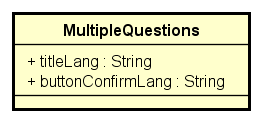
\includegraphics[scale=0.80]{UML/Classi/Front-End/QuizziPedia_Front-end_Views_MultipleQuestionsView.png}
	\caption{QuizziPedia::Front-End::Views::MultipleQuestionsView}
\end{figure} \FloatBarrier
\begin{itemize}
	\item \textbf{Descrizione}: view contenente le direttive per creare una domanda a risposta multipla;
	\item \textbf{Utilizzo}: permette all'utente di creare una domanda a risposta multipla compilando i campi proposti;
	\item \textbf{Relazioni con altre classi}:
		\begin{itemize}
			\item \textit{IN} \texttt{MultipleQuestionsModelView}: classe di tipo modelview la cui istanzazione è contenuta all'interno della variabile di ambiente \$scope di \texttt{Angular.js}. All'interno di essa sono presenti le variabili e i metodi necessari per il \textit{Two-Way Data-Binding\ped{G}} tra la view \texttt{MultipleQuestionsView} e il controller \texttt{MultipleQuestionsController};
			\item \textit{IN} \texttt{TopicKeywordsDirective}: directive che permette di gestire l'inserimento di keywords al momento della creazione della domanda;
			\item \textit{IN} \texttt{ImageInTheQuestionDirective}: directive per l'inserimento dell'immagine nella creazione delle domande;
			\item \textit{IN} \texttt{QuestionTextDirective}: rappresenta il componente grafico che permette all'utente di scrivere o modificare il testo di una domanda;
			\item \textit{IN} \texttt{MultipleChoiceAnswerDirective}: directive contenente il componente grafico per le risposte a scelta;
			\item \textit{IN} \texttt{LangModel}: rappresenta il modello delle informazioni per la giusta traduzione dell'applicazione.
		\end{itemize}
	\item \textbf{Attributi}:
	\begin{itemize}
		\item \texttt{+ titleLangMultiple: String} \\ Attributo che viene utilizzato per visualizzare la giusta traduzione del titolo della pagina, in italiano o in inglese;
		\item \texttt{+ buttonConfirmLangMultiple: String} \\ Attributo che viene utilizzato per visualizzare la giusta traduzione della \textit{label\ped{G}} per il bottone di conferma, in italiano o in inglese;
		\item \texttt{+ buttonLoadImageLang: String} \\ Attributo che viene utilizzato per visualizzare la giusta traduzione della \textit{label\ped{G}} per il bottone di caricamento dell'immagine nel testo della domanda, in italiano o in inglese;
		\item \texttt{+ successCreation: String} \\ Attributo che visualizza un messaggio di conferma avvenuta creazione della domanda;
		\item \texttt{+ errorCreation: String} \\ Attributo che visualizza un messaggio d'errore per la creazione della domanda.
	\end{itemize}
\end{itemize}